\documentclass[twocolumn]{aastex631}

% Package imports go here.

% Local commands go here.

\graphicspath{{./images/}}



\newcommand{\docRef}{PSTN-017}
\newcommand{\docUpstreamLocation}{\url{https://github.com/lsst-pst/pstn-017}}

\providecommand{\secref}[1]{Section~\ref{#1}}
\providecommand{\appref}[1]{Appendix~\ref{#1}}
\providecommand{\partref}[1]{Part~\ref{#1}}
\providecommand{\tabref}[1]{Table~\ref{#1}}
\providecommand{\figref}[1]{Figure~\ref{#1}}
\providecommand{\eqnref}[1]{Eq.~\ref{#1}}


\begin{document}
%% DO NOT EDIT THIS FILE. IT IS GENERATED FROM db2authors.py"
%% Regenerate using:
%%    python $LSST_TEXMF_DIR/bin/db2authors.py > authors.tex


\author[0000-0003-4141-6195]{William~O'Mullane}
\affiliation{Rubin Observatory Project Office, 950 N.\ Cherry Ave., Tucson, AZ  85719, USA}

\author[0000-0003-0800-8755]{Leanne~P.~Guy}
\affiliation{Rubin Observatory Project Office, 950 N.\ Cherry Ave., Tucson, AZ  85719, USA}

\author[0000-0001-9445-1846]{John~D.~Swinbank}
\affiliation{University of Washington, Dept.\ of Astronomy, Box 351580, Seattle, WA 98195, USA}
\affiliation{Department of Astrophysical Sciences, Princeton University, Princeton, NJ 08544, USA}

\author[0000-0002-0558-0521]{Colin~T.~Slater}
\affiliation{University of Washington, Dept.\ of Astronomy, Box 351580, Seattle, WA 98195, USA}


\title{Overview of the Vera C.\ Rubin Observatory Data Management}
\hypersetup{
    pdftitle={Overview of Vera C. Rubin Observatory Data Management},
    pdfauthor={O'Mullane et al},
    pdfkeywords={LSST, Data Management}}


\begin{abstract}
Vera C. Rubin Observatory Data Management (DM) subsystem is one of four construction subsystems.
In operations we retain the notion of four departments of which one is DM.
In this paper we describe DM as built as well as the fabric around DM which enabled its success.
The goal of DM in construction was to "Stand up operable, maintainable, quality services to deliver high-quality LSST data products for science and education, all on time and within reasonable cost."
That said we do outline the data products which will be produced by DM software as a part of the overall Rubin effort.
We refer to detail oriented papers in many areas for the interested reader.

\end{abstract}



\keywords{%
    Astrophysics - Instrumentation and Methods for Astrophysics
    ---
    methods: data analysis
    ---
    methods: miscellaneous
}


\section{Introduction}

Within the Vera C.\ Rubin Observatory \citep{2019ApJ...873..111I} the Data Management (DM) team was tasked to stand up operable, maintainable, quality services to deliver high-quality LSST data products for science and education, all on time and within reasonable cost.
DM is responsible for provided the tools necessary to take the bits generated by the telescope and turn them in to science ready products.

 See also the Rubin Observatory  Data Management System \citep{2017ASPC..512..279J,2022arXiv221113611O}


\subsection{Science Drivers}
The astronomical size and complexity of the expected Rubin data drives many of the architectural choices made for the DM system. The following table highlights some of the key numbers that have influenced choices in DM.

\begin{deluxetable}{llc}
\tablecaption{Rubin Key Numbers driving DM architectural choices\label{tab:dm_keynumbers}}

\tablehead{\colhead{Parameters} & \colhead{Number} & \colhead{Unit}}

\startdata
N Objects & 40 billion & -- \\
N Alerts per image & 10 000 & -- \\
N Alerts per night & 10 million & -- \\
N Images per night & 1000 & -- \\
\enddata

\end{deluxetable}

\subsection{Technical Challenges}
The operational goal of Rubin Observatories Legacy Survey of Space and time is to produce an optical/near-IR survey of half the sky in ugrizy bands to r 27.5 (36 nJy) based on 825 visits over a 10-year period. It is a deep wide fast survey.
Each Rubin image is around 8GB and we take more than one per minute or about 1000 per night.
Add the $\approx$ 450 calibration exposures each day and it means about 20TB of data has to be shipped from Chile to SLAC on a daily basis.
Alerts are to be produced in under 2 minutes with a  goal of doing them in 1 minute which gives us a
challenging transmission and prompt processing time window (see \autoref{sec:dataacquisition}).

Over the 10 year survey we estimate having 2.75M on sky images and at least 1M more calibrations totaling about 50PB.
As we grow this must be reprocessed each year to produce the data releases (see \autoref{sec:dataproduction}.



\section{Organisation of Data Management} \label{sec:org}

The organistion and management of DM is covered in detail in \cite{LDM-294}.


\begin{figure}
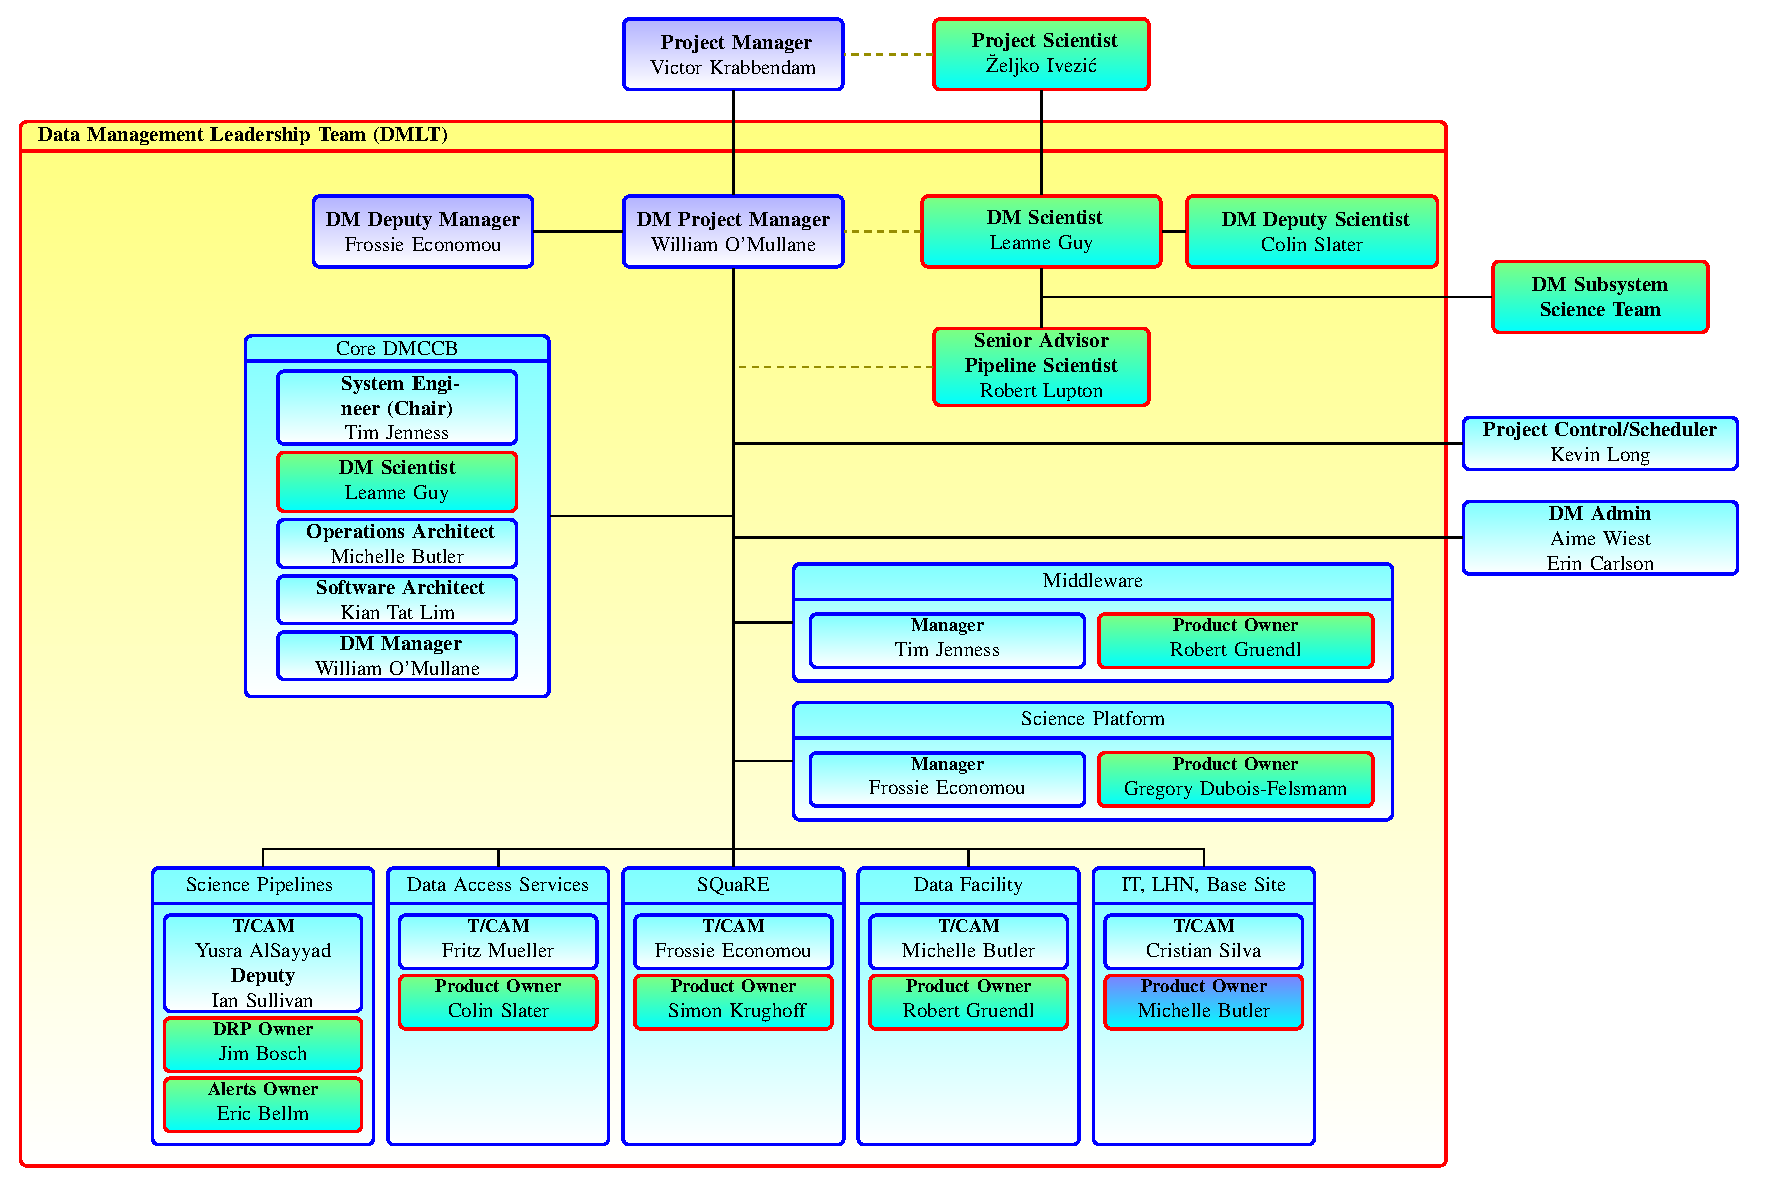
\includegraphics[width=0.6\textwidth]{images/DmOrg}
\caption{\label{fig:org}}
\end{figure}


\subsection{Relationship to other subsystems}
   We take images from the  LSST camera: \cite{2010SPIE.7735E..0JK}

   We are commanded and listen to the  Telescope  and site software  \cite{2014SPIE.9145E..1AG}


   DM will be verified and validated as part of System verification and validation: \cite{2014SPIE.9150E..0NS}

\section {Architecture, Data Transmission and  Access } \label{sec:arch}
DM spans multiple locations with processing occurring at the USDF (SLAC), FrDF (IN2P3) and UK (IRIS).
The system vision has been fairly consistently to deliver science ready data products to the Rubin community as depicted in \autoref{fig:vision}.

\begin{figure*}[ht]
\plotone{DMSystemVision}
\caption{Overview of data management from the telescope to the user. \label{fig:vision}}
\end{figure*}

The organisation and management of DM is covered in \autoref{sec:org}

The DM system architecture was laid out in \cite{LDM-148} from which we reproduce \autoref{fig:arch}
\begin{figure}
\plotone{DMS_Architecture}
\caption{Rubin DM architecture diagram \citet{LDM-148}\label{fig:arch}}
\end{figure}


As shown in \figref{fig:vision} there are several kinds of Rubin data - mostly they are accessed via
the science platform or other services which are described in \autoref{sec:dataservices}.

Data production \autoref{sec:dataproduction} is responsible for all of the pipelines and their execution.

Of course all these services and pipelines must run on hardware which is typically at a data facility.
The data facilities are covered in \autoref{sec:datafacilities}


\subsection{Alerts and Brokers}
Alerts are  product of DM operations and  briefly covered in \autoref{sec:dataproducts}.
The software producing alerts, know and the Alerts Pipeline (AP), is discussed in \todo{REFER TO ALERTS PIPELINES SECTION}
\todo{Leanne: you said you might have a go a this }
Mention community alert brokers.

\section {Software Products} \label{sec:softproduts}
The detailed software approach is covered in \cite{PSTN-019}. Here we go over the main software products.



\subsection{Commissioning Software Products} 
A detailed section describing what we delivered and used to process the commissioning data.
This section will probably not be written until  commissioning.


\subsection{Anticipated Data Release 1 Software Products} 
A short section describing what we anticipate delivering  for DR1 in addition to what was delivered in commissioning. 
This section will probably not be written until after commissioning.

\section{Data Products} \label{sec:dataproducts}

 Rubin Observatory’s LSST Science Pipelines (\S~\ref{sec:softproducts}) will produce the \emph{science-ready data products}.
 These data products have been carefully designed to enable the vast majority of LSST science without the need to access the raw pixels, nor for users to reprocess the data. 
There will however be some science cases where pixel access or a reprocessing of the data is warranted are, such as estimating and subtracting a different background (LSB science), reprocessing a small fraction of images to develop the systematics budget for weak lensing studies (Dark Energy science), or injecting fake objects into images and reprocessing them to develop models for artifact rejection.  
In all such cases involving image reprocessing, we anticipate that users will start from images that have been corrected for instrumental effects and photometrically and astrometrically calibrated. 

The Data Products Definition Document, \citep{LSE-163} was used to  describe the data products produced by the LLSST  and guide the development of the Data Management System.

In this section we provide a high-level overview of the LSST science-ready data products. 
A detailed description of the LSST data products and their scientific performance on the early LSST commissioning data is given in \citep{PSTN-024}.


% Types of data product 
% -- the different types
% Categories of data product
% -- the different categories are designed to address different goals, and are delivered on a range of cadences.

%Describe the science  that they will enable - i.e why are we creating these data products?
%How are they created, how are they distributed and or served

\subsection{Types of Data Product} \label{sec:dp-types}
LSST produces several types of data products. 

\paragraph {\tt Images}~
processed visit images (PVI) are images that have been corrected for instrumental effects and photometrically and astrometrically  calibrated.
raw single visit images, calibrated processed visit images (PVI), coadd images, cutouts (postage stamps)

Include a description of cutout images and how they will be accessed

What is the maximum size of a cutout, how many at a time?

Image data products also includes   calibration frames (darks, flats, biases, fringe, etc.) 

coadds -- We reiterate that not all coadds will be kept and served to the public

template coadds

RGB color images derived from coadds

\paragraph {\tt  Catalogs}~
DR includes Object, Source, DIASource, DIAObject,

Object
`
Source 

ForcedSource

ShearObject

\paragraph {\tt  Alerts}~
A composite data product that includes image cutouts (postage stamps) and extracts of catalog data.
Alerts packets are distributed via the alert distribution system (\S~ref), one alert for each object that 	has changed in brightness or position on the sky.

% 5Sigma alerts


% Sub-threshold alerts
In addition to the alerts detected on DIASources above the nominal detection threshold of 5$\sigma$, we  also measure and store a small sample of DIASources detected the nominal 5$\sigma$ threshold.
There are several drivers  for these \emph{sub-threshold alerts}, for example to enable monitoring of difference image analysis quality or to assess the danger posed by a potentially hazardous asteroid.
A set of criteria, described in \citep{dmtn-228}  was defined  based on key science cases.


\paragraph {\tt  Calibration Data Products} ~
these are images so add to the image section

All auxiliary telescope data, both raw (images with spectra) and processed (calibrated spectra,
derived atmosphere models), will be preserved and made available for download.

All calibration frames (darks, flats, biases, fringe, etc.) will be preserved and made available DMS-REQ-0130
for download as FITS files

\paragraph {\tt  Survey Property Maps}~

Several types of survey property maps will be generated and served to users. 
The properties are typically the mean or total values determined from the images input to generate the deep coadd. 
The types of maps will include the total exposure time; the point-source 5-sigma AB magnitude limit; the weighted mean of the PSF moments; the weighted mean of the sky background and sky noise; and the average effect of differential chromatic refraction (DCR) in the
right ascension and declination directions, and in the PSF moments. 
Property maps based on statistics measured on deep coadds might also be generated.



\subsection{Categories of Data Product} \label{sec:dp-categories}
LSST defines three main categories of data products to be served by Rubin.
The different categories are designed to enable different types of science.
Each category of data product may comprise any or all of the data product types described in \S~\ref{sec:dp-categories}.

% For each category, describe 1) the science that they enable, 2) how they are produced, 3)what the data products in each category are and 4)  how and on what latency they are served. }
% Some general comment somewhere about the various metadata products that are also produced during nightly processing and made available to users.
\subsubsection{Prompt data products} \label{sec:dp-prompt}
Prompt data products are designed to enable time domain science, the rapid discovery, characterization and follow up of objects that have been observed to change in position or brightness on the sky.
{\it Add in a list of science cases that will be enabled on the various time scales}
These data products are fully processed single visit images, difference images, and the catalogs produced by difference image analysis (DIA)  (sec ref to software products).
DIA outputs consist of,  the sources detected in difference images (DIASources), the astrophysical objects that the sources are associated to (DIAObjects),
characterizations of hitherto identified Solar System objects (SSObject), and discoveries of new Solar System objects.

Prompt data products are the result of nightly processing.
Prompt data products are all based on difference imaging, and as such require transient-free templates to  exist for each pointing and filter. The production of templates
Prompt data products are release on a continual and ongoing basis.
Two latencies, 60s for alerts and 24hrs for the catalogs. Data on likely optical transients, will be released publicly with a latency of at most 60s.

They are generated continuously every observing night, including both alerts to objects that have changed brightness or position,
which are released with 60-second latency,
and other catalog and image data products that are released with 24-hour latency.
Prompt image data products include:
\paragraph {Image data products}  PVIs,
\paragraph {Catalog data products}  DIASource, DIAObject catalogs,
\paragraph {Alerts}


\subsubsection{Data Release data products} \label{sec:dp-release}
A Data Release (DR) is specific, fixed {\tt snapshots} of the data at a given time.
Data Releases are made periodically and that can be used and
unambiguously referenced in published analyses.
The catalogs that form the data release will include an extensive list of quantities measured on sources detected in images and
enable a variety of science analyses without the need for users to access or reprocess the images
These data products will be made available as part of an LSST Data Release (\S~???) as the result of coherent
processings of the entire science data set to date.
These will include calibrated images, measurements of positions, fluxes, and shapes,  variability information such as orbital
parameters for moving objects, and an appropriate compact description of light curves.
The Data Release data products will include a uniform reprocessing of the difference imaging-based Prompt data products.

 
\begin{deluxetable*}{lccccc}

%% Keep a portrait orientation
%% \rotate

%% Over-ride the default font size
%% Use Default (12pt)
\tabletypesize{\footnotesize}

%% Use \tablewidth{?pt} to over-ride the default table width.
%% If you are unhappy with the default look at the end of the
%% *.log file to see what the default was set at before adjusting
%% this value.

%% This is the title of the table.
\tablecaption{Summary of LSST Data Products and the cadences on which they will be released}

%% The \tablehead gives provides the column headers.  It
%% is currently set up so that the column labels are on the
%% top line and the units surrounded by ()s are in the
%% bottom line.  You may add more header information by writing
%% another line between these lines. For each column that requries
%% extra information be sure to include a \colhead{text} command
%% and remember to end any extra lines with \\ and include the
%% correct number of &s.
\tablehead{
  \colhead{LSST Data Products} & \multicolumn{3}{c}{Prompt} & \colhead{Data Release} \\
  \colhead{} & \colhead{120 s} & \colhead{<= 24h} & \colhead{>= 80h} & \colhead{Annually}
}

%% All data must appear between the \startdata and \enddata commands
\startdata
Images &  Cutouts in Alerts &   -- &  Single-epoch PVIs  &
      \makecell{Raw exposures (snaps) \\
      Raw exposures (visit)\\
      PVIs \\
      Calibration frames  \\
      Raw \&  processed AuxTel data \\
      Deep coadds \\
      Template coadds \\
      RGB images derived from coadds}
 \\
Catalogs  &   --   &    &    --    &  \\
Alerts    &  \makecell{Alerts to DIASources \\
                       Alerts to sub-threshold DIASources}   &  --   &     --   &    -- \\
Survey Property Maps &    --   &    --  &    --   &  \makecell{Several types of survey property maps}\\
Spectra  &   --   &   --   &     --   &    \makecell{AuxTel spectra} \\
\enddata

%% Include any \tablenotetext{key}{text}, \tablerefs{ref list},
%% or \tablecomments{text} between the \enddata and
%% \end{deluxetable} commands

%% No \tablecomments indicated

%% No \tablerefs indicated

\end{deluxetable*}



\subsection{Other categories of data products}
\label{sec:dpother}

\subsubsection{User Generated data products} \label{sec:dp-user}
User Generated data products data products will originate entirely from the community, including project teams.
These will be created and stored using suitable Application Programming Interfaces (APIs)
that will be provided by the LSST Data Management System.
The system will allow the science teams to use the full power of the Rubin database systems and
Science Platform for the storage, access, and analysis of their results.
It will provide for users and groups to maintain access control over the data products they create,
enabling them to have limited distribution or to be shared with the entire LSST community.

The Rubin Science Platform (\S~???) will allow for the creation of User Generated data
products and will enable science cases that greatly benefit from co-location of
user processing and/or data within the LSST Archive Center.
% SRD

%data products are generated continuously every observing night, including alerts
%to objects that have changed brightness or position.
%
%data products will be made available as annual Data Releases and will include
%images and measurements of positions, fluxes, and shapes, as well as variability information such as orbital parameters for moving objects and an appropriate compact
%description of light curves.

%data products will be created by the community, including project teams, using
%suitable Applications Programming Interfaces (APIs) that will be provided by the LSST
%Data Management System. The Data Management System will also provide at least 10%
%of its total capability for user-dedicated processing and user-dedicated storage. The key
%aspect of these capabilities is that they will reside ?next to" the LSST data, avoiding the
%latency associated with downloads. They will also allow the science teams to use the
%database infrastructure to store their results.


The first two, {\tt Prompt} and {\tt Data Release} data products are produced and delivered by the DM system described in this paper.
The third, {\tt User Generated} data products are produced by the Rubin Science Community using the {\tt Prompt} and {\tt Data Release} together possibly with data from other surveys.

The data product categories are outlined in \citet{LPM-231}

In operations Data Production will use the  software outlined in \secref{sec:softproducts} to produce the various data products.

Show mapping from data product type to category. i.e prompt contains images, catalogs, but not he same ones as DR/

UG catalogs can be federated with DR/PP catalogs.

These data product categories are defined in the SRD \citep{LPM-17} and have been a driver for DM
(add more detail about why)

\subsection{Special programs data products}
Say something about data products from Special Programs.
The special programs data products will be processed and stored as for all other data products.
Maybe doesn't need to be a subsection

\subsection{Custom data products}
During processing, many intermediate data products are created. If is not feasible nor efficient to store them all.
The DM system provides services to generate data products.
Describe the generation of custom data products, in particular to generate  flavours of coadds.




\section {Challenges }
Remaining challenges perhaps ?



\section{Conclusion}





\begin{acknowledgments}
This material is based upon work supported in part by the National Science Foundation through Cooperative Agreement AST-1258333 and Cooperative Support Agreement AST-1202910 managed by the Association of Universities for Research in Astronomy (AURA), and the Department of Energy under Contract No. DE-AC02-76SF00515 with the SLAC National Accelerator Laboratory managed by Stanford University.
Additional Rubin Observatory funding comes from private donations, grants to universities, and in-kind support from LSSTC Institutional Members.
\end{acknowledgments}

\facilities{Rubin (LSSTCam), RubinAux (LATISS)}
\software{
    Rubin Science Platform \citep{LDM-542},
    LSST Science Pipelines \citep{PSTN-019},
    Qserv \citep{Wang:2011:QDS:2063348.2063364}
}

% Include all the relevant bib files.
% https://lsst-texmf.lsst.io/lsstdoc.html#bibliographies
\label{sec:bib}
\bibliography{local,lsst,lsst-dm,refs_ads,refs,books}


\end{document}
